\documentclass[12pt,openright,a4paper]{article}
\setlength{\parindent}{1.3cm}
\setlength{\parskip}{0.2cm}
\usepackage[alf]{abntex2cite}
\usepackage{graphicx}
\usepackage{indentfirst} 
\usepackage{lmodern}
\usepackage{listings}
\pagenumbering{arabic}
\usepackage{lineno}
\usepackage{float}
\linenumbers




\begin{document}
	\linespread{1.5}
 \fontsize{16}{10}\selectfont \centering \textbf{Analysis of computer science newcomers student's motivation} \\
	\fontsize{14}{10}\selectfont {Analysis of student's motivation}\newline

\fontsize{12}{10}
\flushleft
	\textbf{Authors:}\\
	\textbf{Student name:} Felipe Augusto Ferreira de Castro\\
	\textbf{Affiliations:} Federal University of Uberlandia\\
	\textbf{Email:} felipeaugusto.ferreiradecastro@gmail.com \newline
	
\textbf{Professor name:} João Henrique de Souza Pereira\\
\textbf{affiliations:} Federal University of Uberlandia\\
\textbf{email:} joaohs@ufu.br\newline

\textbf{Number of pages:}\\
\textbf{Number of figures:}\\
\textbf{Number of tables:}\\
\textbf{Abstract word number:131,,,,,,}\\
\textbf{introdution word number:}\\
\textbf{discussion word number:}\newline
	
\textbf{Acknowledgments}\\	
My thanks to comppet group that lent me a room to make all data collecting and to all 4 volunteers who made the project possible.\newline

\textbf{conflicts of interest}\footnote{The authors declare no competing financial interests.}

\newpage
\tableofcontents
\newpage
\section{Abstract}
Depression and other mind diseases are currently being reported at universities. Due to it, this research was proposed to observe a group of newcomer students of the Federal University of Uberlândia (UFU) along two semesters. Furthermore ,using resources provided by BCI(Brain computer interface)  technology, to collect an amount of data about their emotional state.

Data collecting were made on 3 points of semester and each one was proposed to the volunteers to do a same activity related to computer science course. They executed those activities  while wearing a EEG based equipment, Epoc+, which was responsible for collecting their emotional data.

The results were satisfying,  students became more stressed along time and their excitement decreased.     Surprisingly relaxation has increased, different from what was expected. The other feelings had no great changes, though.
\section{Significance Statement}
Mental diseases such as depression, stress, anxiety and others, had increased in our society nowadays.  According to World health organization (WHO)  more than 300 million people of all ages suffer from the disease, furthermore , as cited in G1 between 2005 and 2015 in Brazil anxiety cases increased 14,9\% and the country is the first one in related cases of the illness on Latin America, with 5,8\% of the population affected. 

The researcher Michelle Guimarães believes that detecting mental disorders can be a indicator of mental healthiness on young students, also defend that those diseases reduces students productiveness. Due to it, this paper intend to detect the mental mood of students using Brain computer interface and appraise changes along time.      
\section{Introduction}
\section{Materials and Methods}
\subsection{Experimental desing and statistical Analyses}

\section{Results}
 The research has shown satisfactory results. As well as expected, the students stress increased and excitement values of volunteers N1 and N2  reduced along time. The student N3 showed to be a outlier, due to it, the results will be divided by calculus counting N3 and not counting.
 Observing each emotion individually it’s possible to realize that:
 \begin{itemize}
 	\item Stress: It’s one of the most important emotions on this paper and it has shown expected results. Furthermore, its values raised constantly along data collecting with a standard deviation of around 33\% including student N3 and 23\% without N3 values.
 	  \begin{figure}[H]
 	  	\centering
 	  	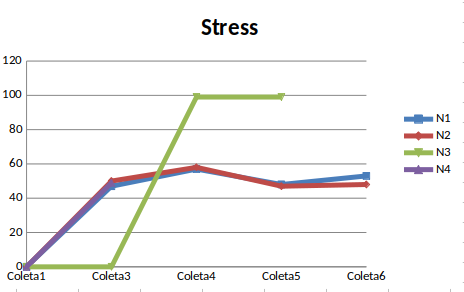
\includegraphics[width=10cm]{./stress.png}
 	  	\caption{students stress values along data collecting}
 	  \end{figure}
 	\item Focus: Behavior of focus was different on each participant, it presented low variance of values from begin of the research until its end, as it is able to be concluded by standard deviation of 11\%.
 	   \begin{figure}[H]
 	  	\centering
 	  	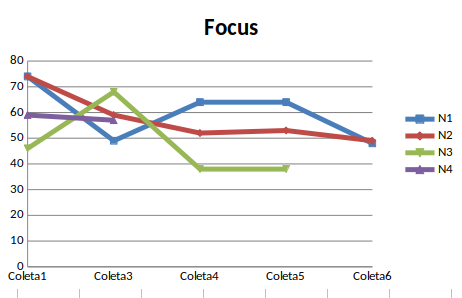
\includegraphics[width=10cm]{./focus.png}
 	  	\caption{students focus values along data collecting}
 	  \end{figure}
 	\item Relaxation: Another important emotion to this paper, which has shown controversial feedback, due to its constant rise of values along data collecting. The emotion has not shown high differences of values, hence standard deviation of it was approximately 7\% without student N3 and around 14\% within N3. 
 	  \begin{figure}[H]
 	 	\centering
 	 	\includegraphics[width=10cm]{./relaxation.png}
 	 	\caption{students relaxation values along data collecting}
 	 \end{figure}
 	\item Interest: Interest comportment  was nearly the same though all data collects. The values of it had little variances and lower standard deviation of all emotions, under 7\% even considering N3 in calculus. 
 	     \begin{figure}[H]
 	    	\centering
 	    	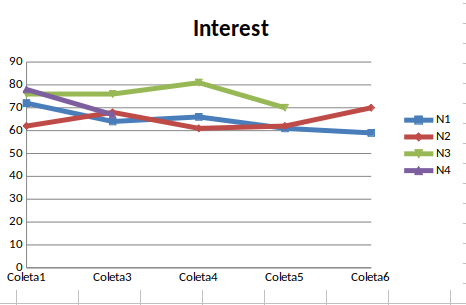
\includegraphics[width=10cm]{./interest.png}
 	    	\caption{students interest values along data collecting}
 	    \end{figure}
 	\item Excitement: This feeling presented high alterations on student N3, a big increase from first data collect to last one, it has shown same lower values in mid term collects though. The standard deviation values was around 14\% considering participant N3 and 12\% without him.
 	      \begin{figure}[H]
 	     	\centering
 	     	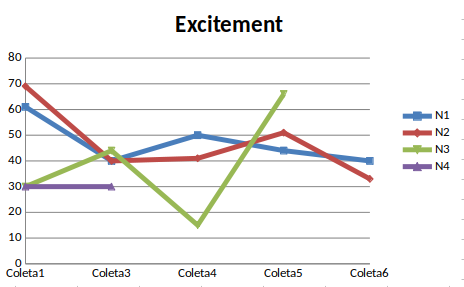
\includegraphics[width=10cm]{./excitement.png}
 	     	\caption{students exitement values along data collecting}
 	     \end{figure}
 	\item Engagement: Students N2 and N4 presented a high difference from collect 1 to 3, that increase was around 56\%. while that, students N1 and N3 did not show significant changes in them values. The general Standard deviation was 21\%,however building groups of students with N1 and N2 being first group and N2 and N4 a second, makes possible to notice that N1 and N3 had no big changes, since standard deviation of the group was 6\%. It is not possible to say same of N2 and N4, because their standard deviation was around 30\%.       
 	    \begin{figure}[H]
 	   	\centering
 	   	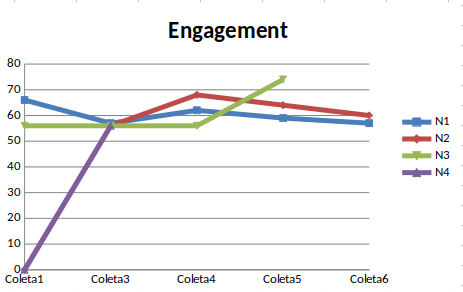
\includegraphics[width=10cm]{./engagement.png}
 	   	\caption{students engagement values along data collecting}
 	   \end{figure}
 \end{itemize}
\section{Discussion}
\section{References}
  G1(2017) Depressão cresce no mundo, segundo OMS; Brasil tem maior prevalência da América Latina (Portuguese). Source:https://g1.globo.com/bemestar/noticia/depressao-cresce-no-mundo-segundo-oms-brasil-tem-maior-prevalencia-da-america-latina.ghtml.\newline
  
  Michelle Guimarães (2014) Depressão,Ansiedade,Estresse e Qualidade de vida dos estudantes de universidade pública e privada (Portuguese).Source: http://tede.metodista.br/jspui/handle/tede/1348 \newline 
  
  World Health Organization(2018) Depression. Source: https://www.who.int/en/news-room/fact-sheets/detail/depression \newline
  
  
\end{document}